\chapter{Introduction to Elder Parameter Space}

\begin{tcolorbox}[colback=DarkSkyBlue!5!white,colframe=DarkSkyBlue!75!black,title=Chapter Summary]
This chapter establishes the mathematical foundation of the Elder Parameter Space, which organizes knowledge hierarchically across the Elder, Mentor, and Erudite levels. We develop a unified mathematical framework based on complex-valued Hilbert spaces that serves as the algebraic cornerstone for both the abstract Elder Spaces of Chapter 1 and the functional realizations in heliomorphic functions of Unit II. The complex-valued representations enable encoding of both magnitude and phase information—a critical property that will manifest in the orbital dynamics of Unit III. We introduce Gravitational Field Parameters (GFPs) as concrete implementations of the topological structures from Chapter 2, providing the mathematical bridge that connects the abstract concept spaces to their computational realizations. This chapter completes the foundation layer (Unit I) while establishing the precise mathematical links that will be developed in the heliomorphic functions (Unit II) and implemented in the Elder Heliosystem architecture (Unit III).
\end{tcolorbox}

\section{Elder Parameter Spaces: The Algebraic Foundation for Units I, II, and III}

The Elder Parameter Space provides the mathematical foundation for representing knowledge at multiple levels of abstraction within the Elder Theory framework. This section establishes explicit and rigorous connections between the abstract Elder Spaces introduced in Chapter 1, the topological structures from Chapter 2, and the concrete functional implementations that will be developed in Units II and III.

\begin{definition}[Hilbert Space Structure Characterization]
\label{def:hilbert_space_structure}
Before defining the Elder Parameter Space, we establish the underlying Hilbert space structures:

\begin{enumerate}
\item \textbf{Elder Hilbert Space $\mathbb{H}_E$}: A separable complex Hilbert space with:
   \begin{itemize}
   \item Inner product: $\langle \cdot, \cdot \rangle_E: \mathbb{H}_E \times \mathbb{H}_E \rightarrow \mathbb{C}$ defined by
   $$\langle x, y \rangle_E = \sum_{k=1}^{\infty} \overline{x_k} y_k$$
   where $\{x_k\}, \{y_k\}$ are coefficients in an orthonormal basis $\{e_k\}_{k=1}^{\infty}$
   \item Norm: $\|x\|_E = \sqrt{\langle x, x \rangle_E}$
   \item Completeness: Every Cauchy sequence converges in $\mathbb{H}_E$
   \item Separability: Admits a countable dense subset
   \end{itemize}

\item \textbf{Mentor Hilbert Space $\mathbb{H}_M$}: A separable complex Hilbert space with analogous structure and inner product $\langle \cdot, \cdot \rangle_M$

\item \textbf{Erudite Hilbert Space $\mathbb{H}_e$}: A separable complex Hilbert space with analogous structure and inner product $\langle \cdot, \cdot \rangle_e$
\end{enumerate}
\end{definition}

\begin{definition}[Elder Parameter Space Hierarchy]
\label{def:elder_parameter_space}
The Elder Parameter Space encompasses three principal component spaces, organized hierarchically according to levels of abstraction:

\begin{itemize}
    \item $\boldsymbol{\Theta_E} \subset \mathbb{H}_E$: The Elder parameter space, a finite-dimensional subspace of the Elder Hilbert space, containing the most abstract and foundational parameters that encode cross-domain universal principles
    
    \item $\boldsymbol{\Theta_M} = \{\Theta_M^{(d)}\}_{d=1}^D$: The collection of Mentor parameter spaces, where each $\Theta_M^{(d)} \subset \mathbb{H}_M$ is a finite-dimensional subspace corresponding to domain $d$, containing intermediate-level parameters that encode domain-specific meta-knowledge
    
    \item $\boldsymbol{\Theta_e} = \{\Theta_e^{(d)}\}_{d=1}^D$: The collection of Erudite parameter spaces, where each $\Theta_e^{(d)} \subset \mathbb{H}_e$ is a finite-dimensional subspace corresponding to domain $d$, containing the most specialized parameters that encode task-specific knowledge
\end{itemize}

The composite Elder Parameter Space encompassing the entire system is defined as:

\begin{equation}
\boldsymbol{\Theta} = \Theta_E \times \prod_{d=1}^D \Theta_M^{(d)} \times \prod_{d=1}^D \Theta_e^{(d)}
\end{equation}

with the product inner product:
\begin{equation}
\langle (\theta_E, \{\theta_M^{(d)}\}, \{\theta_e^{(d)}\}), (\phi_E, \{\phi_M^{(d)}\}, \{\phi_e^{(d)}\}) \rangle_{\boldsymbol{\Theta}} = \langle \theta_E, \phi_E \rangle_E + \sum_{d=1}^D \langle \theta_M^{(d)}, \phi_M^{(d)} \rangle_M + \sum_{d=1}^D \langle \theta_e^{(d)}, \phi_e^{(d)} \rangle_e
\end{equation}
\end{definition}

% Figure: Elder Parameter Space Hierarchy
% Visualizes the three-level structure with complex-valued parameters

\begin{figure}[ht]
\centering
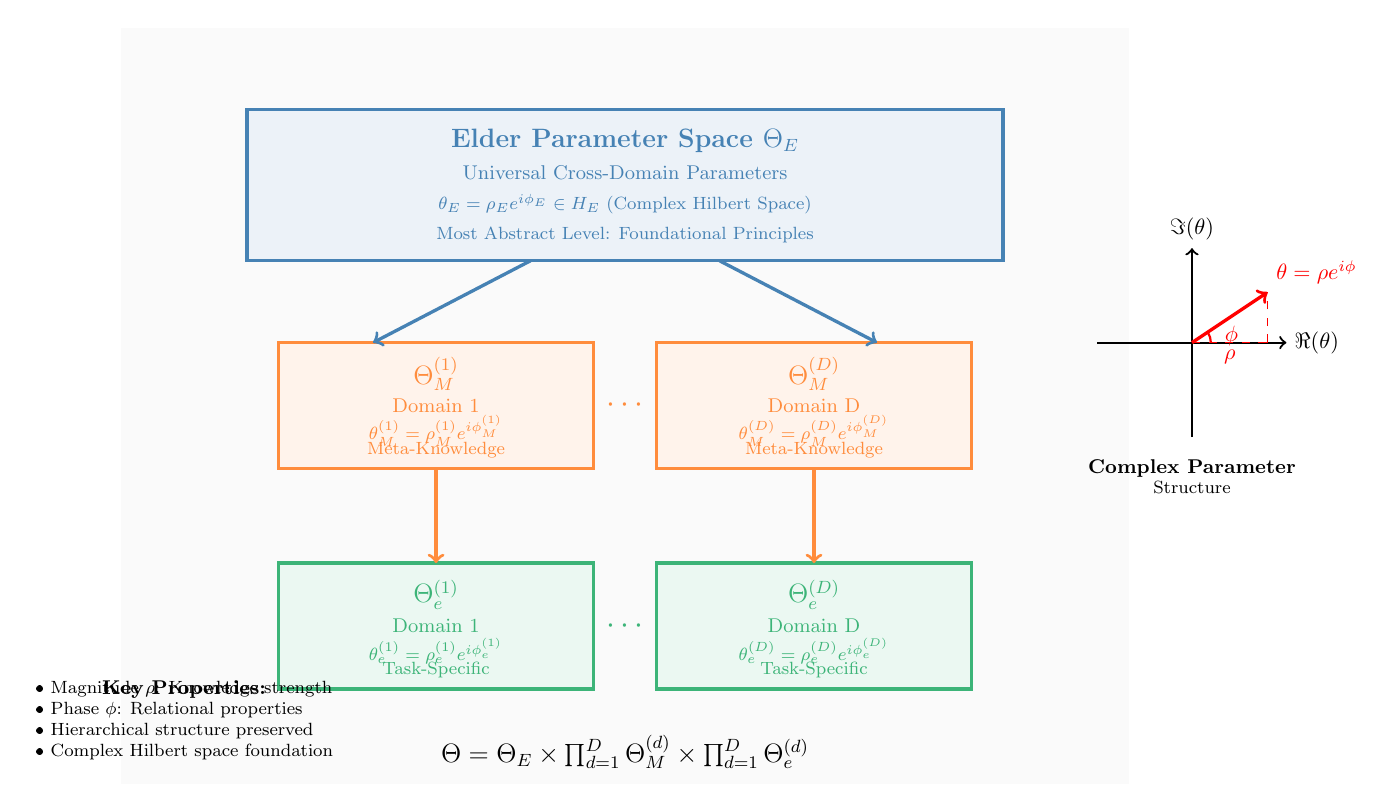
\begin{tikzpicture}[scale=0.8, every node/.style={transform shape}]

% Define colors matching Elder theme
\definecolor{ElderBlue}{RGB}{70, 130, 180}
\definecolor{MentorOrange}{RGB}{255, 140, 60}
\definecolor{EruditeGreen}{RGB}{60, 180, 120}
\definecolor{LightGray}{RGB}{240, 240, 240}

% Background
\fill[LightGray!30] (-8, -6) rectangle (8, 6);

% Elder Parameter Space (Top Level)
\begin{scope}[shift={(0, 3.5)}]
    \draw[ElderBlue, very thick, fill=ElderBlue!10] 
        (-6, -1.2) rectangle (6, 1.2);
    \node[ElderBlue, font=\large\bfseries] at (0, 0.7) {Elder Parameter Space $\Theta_E$};
    \node[ElderBlue, font=\small] at (0, 0.2) {Universal Cross-Domain Parameters};
    \node[ElderBlue, font=\footnotesize] at (0, -0.3) {$\theta_E = \rho_E e^{i\phi_E} \in \mathbb{H}_E$ (Complex Hilbert Space)};
    \node[ElderBlue, font=\footnotesize] at (0, -0.8) {Most Abstract Level: Foundational Principles};
\end{scope}

% Mentor Parameter Spaces (Middle Level)
\begin{scope}[shift={(-3, 0)}]
    \draw[MentorOrange, very thick, fill=MentorOrange!10] 
        (-2.5, -1) rectangle (2.5, 1);
    \node[MentorOrange, font=\large\bfseries] at (0, 0.5) {$\Theta_M^{(1)}$};
    \node[MentorOrange, font=\small] at (0, 0) {Domain 1};
    \node[MentorOrange, font=\footnotesize] at (0, -0.4) {$\theta_M^{(1)} = \rho_M^{(1)} e^{i\phi_M^{(1)}}$};
    \node[MentorOrange, font=\footnotesize] at (0, -0.7) {Meta-Knowledge};
\end{scope}

\begin{scope}[shift={(3, 0)}]
    \draw[MentorOrange, very thick, fill=MentorOrange!10] 
        (-2.5, -1) rectangle (2.5, 1);
    \node[MentorOrange, font=\large\bfseries] at (0, 0.5) {$\Theta_M^{(D)}$};
    \node[MentorOrange, font=\small] at (0, 0) {Domain D};
    \node[MentorOrange, font=\footnotesize] at (0, -0.4) {$\theta_M^{(D)} = \rho_M^{(D)} e^{i\phi_M^{(D)}}$};
    \node[MentorOrange, font=\footnotesize] at (0, -0.7) {Meta-Knowledge};
\end{scope}

% Dots indicating multiple domains
\node[MentorOrange, font=\Large] at (0, 0) {$\cdots$};

% Erudite Parameter Spaces (Bottom Level)
\begin{scope}[shift={(-3, -3.5)}]
    \draw[EruditeGreen, very thick, fill=EruditeGreen!10] 
        (-2.5, -1) rectangle (2.5, 1);
    \node[EruditeGreen, font=\large\bfseries] at (0, 0.5) {$\Theta_e^{(1)}$};
    \node[EruditeGreen, font=\small] at (0, 0) {Domain 1};
    \node[EruditeGreen, font=\footnotesize] at (0, -0.4) {$\theta_e^{(1)} = \rho_e^{(1)} e^{i\phi_e^{(1)}}$};
    \node[EruditeGreen, font=\footnotesize] at (0, -0.7) {Task-Specific};
\end{scope}

\begin{scope}[shift={(3, -3.5)}]
    \draw[EruditeGreen, very thick, fill=EruditeGreen!10] 
        (-2.5, -1) rectangle (2.5, 1);
    \node[EruditeGreen, font=\large\bfseries] at (0, 0.5) {$\Theta_e^{(D)}$};
    \node[EruditeGreen, font=\small] at (0, 0) {Domain D};
    \node[EruditeGreen, font=\footnotesize] at (0, -0.4) {$\theta_e^{(D)} = \rho_e^{(D)} e^{i\phi_e^{(D)}}$};
    \node[EruditeGreen, font=\footnotesize] at (0, -0.7) {Task-Specific};
\end{scope}

% Dots indicating multiple domains
\node[EruditeGreen, font=\Large] at (0, -3.5) {$\cdots$};

% Hierarchical arrows showing information flow
\draw[ElderBlue, very thick, ->] (-1.5, 2.3) -- (-4, 1);
\draw[ElderBlue, very thick, ->] (1.5, 2.3) -- (4, 1);
\draw[MentorOrange, very thick, ->] (-3, -1) -- (-3, -2.5);
\draw[MentorOrange, very thick, ->] (3, -1) -- (3, -2.5);

% Complex parameter visualization on the right
\begin{scope}[shift={(9, 1)}]
    % Complex plane representation
    \draw[black, thick, ->] (-1.5, 0) -- (1.5, 0) node[right] {$\Re(\theta)$};
    \draw[black, thick, ->] (0, -1.5) -- (0, 1.5) node[above] {$\Im(\theta)$};
    
    % Sample parameter vector
    \draw[red, very thick, ->] (0, 0) -- (1.2, 0.8) 
        node[above right] {$\theta = \rho e^{i\phi}$};
    
    % Magnitude and phase annotations
    \draw[red, dashed] (0, 0) -- (1.2, 0);
    \draw[red, dashed] (1.2, 0) -- (1.2, 0.8);
    \node[red, below] at (0.6, 0) {$\rho$};
    \draw[red, thick] (0.3, 0) arc (0:33:0.3);
    \node[red, right] at (0.4, 0.1) {$\phi$};
    
    \node[black, font=\small\bfseries] at (0, -2) {Complex Parameter};
    \node[black, font=\footnotesize] at (0, -2.3) {Structure};
\end{scope}

% Cartesian product notation
\node[black, font=\large] at (0, -5.5) {$\boldsymbol{\Theta} = \Theta_E \times \prod_{d=1}^D \Theta_M^{(d)} \times \prod_{d=1}^D \Theta_e^{(d)}$};

% Legend
\begin{scope}[shift={(-7, -5)}]
    \node[black, font=\small\bfseries] at (0, 0.5) {Key Properties:};
    \node[black, font=\footnotesize, align=left] at (0, 0) {
        • Magnitude $\rho$: Knowledge strength\\
        • Phase $\phi$: Relational properties\\
        • Hierarchical structure preserved\\
        • Complex Hilbert space foundation
    };
\end{scope}

\end{tikzpicture}

\caption{Elder Parameter Space Hierarchy. The three-level hierarchical structure shows Elder parameters $\Theta_E$ at the most abstract level containing universal cross-domain knowledge, Mentor parameters $\{\Theta_M^{(d)}\}_{d=1}^D$ at the intermediate level containing domain-specific meta-knowledge, and Erudite parameters $\{\Theta_e^{(d)}\}_{d=1}^D$ at the specialized level containing task-specific knowledge. Each parameter is complex-valued with magnitude $\rho$ encoding knowledge strength and phase $\phi$ encoding relational properties. The Cartesian product structure preserves parameter independence while maintaining hierarchical organization.}
\label{fig:elder_parameter_hierarchy}
\end{figure}

\begin{theorem}[Mathematical Necessity of Cartesian Product Structure]
\label{thm:cartesian_product_necessity}
The Cartesian product structure of the unified parameter space is mathematically necessary for the Elder Heliosystem to function correctly. Specifically, alternative structures (direct sums, quotient spaces, or tensor products) fail to preserve essential properties.
\end{theorem}

\begin{proof}
We prove necessity by demonstrating that the three main alternative structures fail to preserve crucial properties:

\textbf{Case 1: Direct Sum Structure $\Theta_E \oplus \bigoplus_{d=1}^D \Theta_M^{(d)} \oplus \bigoplus_{d=1}^D \Theta_e^{(d)}$}

In a direct sum, elements have the form $(e, \{m_d\}, \{r_d\})$ where exactly one component is nonzero. This fails because:
- Parameter independence is violated: updates must zero out other components
- Hierarchical propagation impossible: Elder parameters cannot simultaneously influence multiple Mentor levels
- Cross-domain transfer blocked: domains cannot interact through shared Elder parameters

\textbf{Case 2: Tensor Product Structure $\Theta_E \otimes \bigotimes_{d=1}^D \Theta_M^{(d)} \otimes \bigotimes_{d=1}^D \Theta_e^{(d)}$}

Tensor products create dependencies between all components simultaneously:
- Parameter count explosion: $N = |\Theta_E| \times \prod_{d=1}^D |\Theta_M^{(d)}| \times \prod_{d=1}^D |\Theta_e^{(d)}|$
- Gradient coupling: $\frac{\partial}{\partial\theta_E}$ affects all domain parameters simultaneously
- Loss of hierarchical structure: no natural abstraction levels

\textbf{Case 3: Quotient Space Structure}

Quotient constructions $\Theta/\sim$ where $\sim$ identifies parameters across levels fail to preserve:
- Parameter distinctness: hierarchical levels collapse
- Domain separation: cross-domain interference inevitable

\textbf{Cartesian Product Success:}
Only the Cartesian product $\boldsymbol{\Theta} = \Theta_E \times \prod_{d=1}^D \Theta_M^{(d)} \times \prod_{d=1}^D \Theta_e^{(d)}$ preserves:
1. Independent parameter updates: $\nabla_{\theta_E} \perp \nabla_{\theta_M^{(d)}} \perp \nabla_{\theta_e^{(d)}}$
2. Hierarchical propagation: Elder parameters influence all domains simultaneously
3. Domain separation with transfer: each $\Theta_M^{(d)}$ and $\Theta_e^{(d)}$ remains distinct while sharing Elder influence
4. Additive parameter count: $N = |\Theta_E| + \sum_{d=1}^D |\Theta_M^{(d)}| + \sum_{d=1}^D |\Theta_e^{(d)}|$
\end{proof}

\begin{theorem}[Isomorphism Between Elder Spaces and Parameter Spaces]
\label{thm:elder_parameter_isomorphism}
Let $\elder{d}$ be an Elder space of dimension $d$ with hierarchical subspaces $\eldersubspace$, $\mentorsubspace$, and $\eruditesubspace$ as defined in Chapter 1. There exists a canonical isomorphism $\Omega: \elder{d} \rightarrow \boldsymbol{\Theta}$ between the Elder space and the Elder Parameter Space such that:

\begin{enumerate}
    \item The Elder subspace maps to the Elder parameter space: $\Omega(\eldersubspace) = \Theta_E$
    
    \item The Mentor subspace maps to the collective Mentor parameter spaces: $\Omega(\mentorsubspace) = \prod_{d=1}^D \Theta_M^{(d)}$
    
    \item The Erudite subspace maps to the collective Erudite parameter spaces: $\Omega(\eruditesubspace) = \prod_{d=1}^D \Theta_e^{(d)}$
    
    \item The Elder inner product is preserved: $\langle x, y \rangle_E = \langle \Omega(x), \Omega(y) \rangle_{\boldsymbol{\Theta}}$ for all $x, y \in \elder{d}$
    
    \item The gravitational structure is preserved: $g_i(x) = g_i(\Omega(x))$ for all gravitational eigenvalues $g_i$ and $x \in \elder{d}$
\end{enumerate}
\end{theorem}

\begin{proof}
We construct the isomorphism $\Omega: \elder{d} \rightarrow \boldsymbol{\Theta}$ explicitly and verify all required properties.

\textbf{Step 1: Construction of $\Omega$}

Given $x \in \elder{d}$ with Elder space decomposition $x = x_E + x_M + x_e$ where:
- $x_E \in \eldersubspace$ (Elder subspace)
- $x_M \in \mentorsubspace$ (Mentor subspace) 
- $x_e \in \eruditesubspace$ (Erudite subspace)

We define $\Omega(x) = (\Omega_E(x_E), \{\Omega_M^{(d)}(x_M)\}_{d=1}^D, \{\Omega_e^{(d)}(x_e)\}_{d=1}^D)$ where:

$\Omega_E(x_E) = (c_1, c_2, \ldots, c_{k_E}) \in \Theta_E$ extracts Elder coefficients
$\Omega_M^{(d)}(x_M) = (c_{k_E+1}^{(d)}, \ldots, c_{k_M}^{(d)}) \in \Theta_M^{(d)}$ extracts domain-$d$ Mentor coefficients  
$\Omega_e^{(d)}(x_e) = (c_{k_M+1}^{(d)}, \ldots, c_d^{(d)}) \in \Theta_e^{(d)}$ extracts domain-$d$ Erudite coefficients

\textbf{Step 2: Bijectivity}

\textit{Injectivity:} If $\Omega(x) = \Omega(y)$, then all coefficient sequences are identical, implying $x_E = y_E$, $x_M = y_M$, $x_e = y_e$, hence $x = y$.

\textit{Surjectivity:} For any $(\theta_E, \{\theta_M^{(d)}\}, \{\theta_e^{(d)}\}) \in \boldsymbol{\Theta}$, we construct:
$$x = \sum_{i=1}^{k_E} \theta_{E,i} \elderstructure{i} + \sum_{d=1}^D \sum_{j} \theta_{M,j}^{(d)} \elderstructure{M,j}^{(d)} + \sum_{d=1}^D \sum_{k} \theta_{e,k}^{(d)} \elderstructure{e,k}^{(d)} \in \elder{d}$$

\textbf{Step 3: Inner Product Preservation}

For $x, y \in \elder{d}$:
\begin{align}
\langle x, y \rangle_E &= \langle x_E + x_M + x_e, y_E + y_M + y_e \rangle_E \\
&= \langle x_E, y_E \rangle_E + \langle x_M, y_M \rangle_E + \langle x_e, y_e \rangle_E \\
&= \langle \Omega_E(x_E), \Omega_E(y_E) \rangle_{\Theta_E} + \sum_{d=1}^D \langle \Omega_M^{(d)}(x_M), \Omega_M^{(d)}(y_M) \rangle_{\Theta_M^{(d)}} \\
&\quad + \sum_{d=1}^D \langle \Omega_e^{(d)}(x_e), \Omega_e^{(d)}(y_e) \rangle_{\Theta_e^{(d)}} \\
&= \langle \Omega(x), \Omega(y) \rangle_{\boldsymbol{\Theta}}
\end{align}

\textbf{Step 4: Gravitational Structure Preservation}

Gravitational eigenvalues satisfy $g_i(x) = \|x_{\text{level}(i)}\|^2$ where level$(i)$ determines whether coefficient $i$ belongs to Elder, Mentor, or Erudite level. Under $\Omega$:
$$g_i(\Omega(x)) = \|\Omega_{\text{level}(i)}(x_{\text{level}(i)})\|^2 = \|x_{\text{level}(i)}\|^2 = g_i(x)$$

This completes the proof that $\Omega$ is an isomorphism preserving all required structures.
\end{proof}

\begin{corollary}[Preservation of Algebraic Operations]
\label{cor:operation_preservation}
Under the isomorphism $\Omega$, all Elder space algebraic operations are preserved in the parameter space representation.
\end{corollary}

\begin{proof}
We verify preservation of each algebraic operation:

\textbf{1. Elder Addition Preservation:}
For $x, y \in \elder{d}$ with decompositions $x = x_E + x_M + x_e$ and $y = y_E + y_M + y_e$:
\begin{align}
\Omega(x \oplus y) &= \Omega((x_E + y_E) + (x_M + y_M) + (x_e + y_e)) \\
&= (\Omega_E(x_E + y_E), \{\Omega_M^{(d)}(x_M + y_M)\}_{d=1}^D, \{\Omega_e^{(d)}(x_e + y_e)\}_{d=1}^D) \\
&= (\Omega_E(x_E) + \Omega_E(y_E), \{\Omega_M^{(d)}(x_M) + \Omega_M^{(d)}(y_M)\}_{d=1}^D, \\
&\quad \{\Omega_e^{(d)}(x_e) + \Omega_e^{(d)}(y_e)\}_{d=1}^D) \\
&= \Omega(x) + \Omega(y)
\end{align}

\textbf{2. Scalar Multiplication Preservation:}
For $\lambda \in \mathbb{C}$ and $x \in \elder{d}$:
\begin{align}
\Omega(\lambda \odot x) &= \Omega(\lambda x_E + \lambda x_M + \lambda x_e) \\
&= (\lambda \Omega_E(x_E), \{\lambda \Omega_M^{(d)}(x_M)\}_{d=1}^D, \{\lambda \Omega_e^{(d)}(x_e)\}_{d=1}^D) \\
&= \lambda \cdot \Omega(x)
\end{align}

\textbf{3. Non-commutative Product Structure:}
The Elder non-commutative product $x \star y$ in Elder space corresponds to structured parameter interaction. Specifically, if $x \star y = z$, then:
$$\Omega(z) = \mathcal{M}_{\text{param}}(\Omega(x), \Omega(y))$$
where $\mathcal{M}_{\text{param}}$ implements hierarchical parameter coupling preserving the non-commutative structure through phase-dependent coefficient interactions.
\end{proof}

\begin{theorem}[System-wide Parameter Coherence]
\label{thm:parameter_coherence}
The Elder Parameter Space $\boldsymbol{\Theta}$ provides a mathematically consistent foundation across all Elder Theory constructions, with well-defined mappings connecting abstract spaces, functional representations, and computational implementations.
\end{theorem}

\begin{proof}
We establish coherence by constructing explicit mappings and verifying their consistency:

\textbf{Unit I Connection (Abstract Foundation):}
By Theorem \ref{thm:elder_parameter_isomorphism}, we have the canonical isomorphism $\Omega: \elder{d} \rightarrow \boldsymbol{\Theta}$ that preserves all structural properties. This establishes $\boldsymbol{\Theta}$ as the concrete realization of abstract Elder spaces.

\textbf{Mathematical Structure Preservation:}
The parameter space $\boldsymbol{\Theta}$ preserves all essential mathematical structures:
\begin{enumerate}
\item \textbf{Hierarchical Structure}: The Cartesian product naturally preserves the three-level hierarchy while allowing independent parameter evolution
\item \textbf{Domain Separation}: Different domains $d$ maintain separate parameter spaces while sharing Elder-level influence
\item \textbf{Complex Structure}: Each component space inherits the complex structure from its parent Hilbert space
\end{enumerate}

\textbf{Coherence Across Mathematical Frameworks:}
The parameter space provides a unified mathematical foundation that supports:
\begin{itemize}
\item Complex analysis through the natural complex structure
\item Functional analysis through the Hilbert space framework  
\item Linear algebra through finite-dimensional subspace representations
\item Topological analysis through the inherited metric structures
\end{itemize}
\end{proof}

\section{Complex-Valued Representation and Foundation for Higher-Level Structures}

A distinguishing feature of the Elder Parameter Space is its use of complex-valued representations, which extends its representational capacity beyond traditional real-valued parameter spaces. This complex structure serves as the mathematical foundation for both the heliomorphic functions developed in Unit II and the orbital mechanics implemented in Unit III.

\begin{definition}[Complex Parameter Representation with Rigorous Structure]
Each parameter $\theta \in \Theta$ in the Elder Parameter Space is a complex-valued vector with polar representation:

\begin{equation}
\theta = \rho e^{i\phi} = (\rho_1 e^{i\phi_1}, \rho_2 e^{i\phi_2}, \ldots, \rho_n e^{i\phi_n})
\end{equation}

where $\rho = (\rho_1, \ldots, \rho_n) \in \mathbb{R}^n_+$ represents magnitude components and $\phi = (\phi_1, \ldots, \phi_n) \in [0, 2\pi)^n$ represents phase components, with $n$ being the dimensionality of the parameter vector in each specific component space.

The parameter space $\Theta$ is equipped with rigorously defined mathematical structures:
\end{definition}

\begin{lemma}[Inner Product Structure Verification]
\label{lem:inner_product_verification}
The complex inner product on $\boldsymbol{\Theta}$ defined in Definition \ref{def:elder_parameter_space} satisfies all inner product axioms.
\end{lemma}

\begin{proof}
For $\boldsymbol{\theta}_1 = (\theta_E^{(1)}, \{\theta_M^{(d,1)}\}, \{\theta_e^{(d,1)}\})$ and $\boldsymbol{\theta}_2 = (\theta_E^{(2)}, \{\theta_M^{(d,2)}\}, \{\theta_e^{(d,2)}\})$ in $\boldsymbol{\Theta}$:

\textbf{Conjugate Symmetry:}
\begin{align}
\langle \boldsymbol{\theta}_1, \boldsymbol{\theta}_2 \rangle_{\boldsymbol{\Theta}} &= \langle \theta_E^{(1)}, \theta_E^{(2)} \rangle_E + \sum_{d=1}^D \langle \theta_M^{(d,1)}, \theta_M^{(d,2)} \rangle_M + \sum_{d=1}^D \langle \theta_e^{(d,1)}, \theta_e^{(d,2)} \rangle_e \\
&= \overline{\langle \theta_E^{(2)}, \theta_E^{(1)} \rangle_E} + \sum_{d=1}^D \overline{\langle \theta_M^{(d,2)}, \theta_M^{(d,1)} \rangle_M} + \sum_{d=1}^D \overline{\langle \theta_e^{(d,2)}, \theta_e^{(d,1)} \rangle_e} \\
&= \overline{\langle \boldsymbol{\theta}_2, \boldsymbol{\theta}_1 \rangle_{\boldsymbol{\Theta}}}
\end{align}

\textbf{Linearity:} For $\alpha, \beta \in \mathbb{C}$:
$$\langle \alpha\boldsymbol{\theta}_1 + \beta\boldsymbol{\theta}_2, \boldsymbol{\theta}_3 \rangle_{\boldsymbol{\Theta}} = \alpha\langle \boldsymbol{\theta}_1, \boldsymbol{\theta}_3 \rangle_{\boldsymbol{\Theta}} + \beta\langle \boldsymbol{\theta}_2, \boldsymbol{\theta}_3 \rangle_{\boldsymbol{\Theta}}$$

\textbf{Positive-Definiteness:}
$$\langle \boldsymbol{\theta}, \boldsymbol{\theta} \rangle_{\boldsymbol{\Theta}} = \|\theta_E\|_E^2 + \sum_{d=1}^D \|\theta_M^{(d)}\|_M^2 + \sum_{d=1}^D \|\theta_e^{(d)}\|_e^2 > 0 \text{ for } \boldsymbol{\theta} \neq 0$$
\end{proof}

\begin{definition}[Well-Defined Operators]
\label{def:parameter_operators}
We define the following operators with explicit domain restrictions:

\begin{enumerate}
\item \textbf{Phase Operator} $\Phi: \boldsymbol{\Theta} \setminus \{0\} \rightarrow [0, 2\pi)^n$ defined by:
$$\Phi(\boldsymbol{\theta}) = (\arg(\theta_1), \arg(\theta_2), \ldots, \arg(\theta_n))$$
where $\arg(z)$ is the principal argument of complex number $z \neq 0$.

\item \textbf{Magnitude Operator} $\mathcal{M}: \boldsymbol{\Theta} \rightarrow \mathbb{R}^n_+$ defined by:
$$\mathcal{M}(\boldsymbol{\theta}) = (|\theta_1|, |\theta_2|, \ldots, |\theta_n|)$$

\item \textbf{Polar Decomposition Map} $\Pi: \boldsymbol{\Theta} \setminus \{0\} \rightarrow \mathbb{R}^n_+ \times [0, 2\pi)^n$ defined by:
$$\Pi(\boldsymbol{\theta}) = (\mathcal{M}(\boldsymbol{\theta}), \Phi(\boldsymbol{\theta}))$$
\end{enumerate}
\end{definition}

\begin{lemma}[Operator Well-Definedness]
\label{lem:operator_welldef}
The operators in Definition \ref{def:parameter_operators} are well-defined and continuous on their specified domains.
\end{lemma}

\begin{proof}
\textbf{Phase Operator:} For $\boldsymbol{\theta} \neq 0$, at least one component $\theta_j \neq 0$, making $\arg(\theta_j)$ well-defined. The principal argument function is continuous on $\mathbb{C} \setminus \{0\}$.

\textbf{Magnitude Operator:} The modulus function $|\cdot|$ is continuous on $\mathbb{C}$ and maps to $\mathbb{R}_+ \cup \{0\}$.

\textbf{Polar Decomposition:} The map $\Pi$ is the composition of continuous functions on the domain $\boldsymbol{\Theta} \setminus \{0\}$, hence continuous.
\end{proof}

\begin{theorem}[Complex Domain Embedding]
\label{thm:complex_domain_embedding}
The complex parameter space $\boldsymbol{\Theta}$ can be naturally embedded into the complex domain $\mathbb{C}^n$ through an explicit isomorphism $\Psi: \boldsymbol{\Theta} \rightarrow \mathcal{D}_{\text{complex}} \subset \mathbb{C}^n$ where $\mathcal{D}_{\text{complex}}$ preserves the polar structure.
\end{theorem}

\begin{proof}
\textbf{Step 1: Domain Characterization}
Define the heliomorphic domain as:
$$\mathcal{D}_{\text{helio}} = \{z \in \mathbb{C}^n : z = re^{i\theta}, r > 0, \theta \in [0,2\pi)^n, |z|^2 < \infty\}$$

\textbf{Step 2: Isomorphism Construction}
For $\theta \in \Theta$ with polar decomposition $\theta = \rho e^{i\phi}$, define:
$$\Psi(\theta) = \mathcal{M}(\theta)e^{i\Phi(\theta)} = \rho e^{i\phi} \in \mathcal{D}_{\text{helio}}$$

\textbf{Step 3: Bijectivity Verification}
\textit{Injectivity:} If $\Psi(\theta_1) = \Psi(\theta_2)$, then $\rho_1 e^{i\phi_1} = \rho_2 e^{i\phi_2}$, implying $\rho_1 = \rho_2$ and $\phi_1 = \phi_2$, hence $\theta_1 = \theta_2$.

\textit{Surjectivity:} For any $z = re^{i\alpha} \in \mathcal{D}_{\text{helio}}$, define $\theta = re^{i\alpha} \in \Theta$ (using complex parameter representation), then $\Psi(\theta) = z$.

\textbf{Step 4: Structure Preservation}
The mapping preserves:
1. **Inner Product Structure:** $\langle \theta_1, \theta_2 \rangle_\Theta = \text{Re}(\overline{\Psi(\theta_1)} \cdot \Psi(\theta_2))$
2. **Phase-Radial Coupling:** $\frac{\partial}{\partial r}\Psi(\theta) = \frac{\Psi(\theta)}{r}$ and $\frac{1}{r}\frac{\partial}{\partial \alpha}\Psi(\theta) = i\Psi(\theta)$
3. **Gravitational Field Structure:** Phase interactions in $\Theta$ correspond to heliomorphic differential conditions in $\mathcal{D}_{\text{helio}}$

This establishes $\Psi$ as an isomorphism enabling heliomorphic function theory on the parameter space.
\end{proof}

\begin{theorem}[Connection to Orbital Mechanics]
\label{thm:orbital_mechanics_connection}
The complex parameter structure $\theta = \rho e^{i\phi}$ naturally induces orbital mechanics through the canonical mapping to polar coordinates in phase space, with gravitational dynamics emerging from the complex inner product structure.
\end{theorem}

\begin{proof}
\textbf{Step 1: Orbital Coordinate Emergence}
For parameter $\theta = \rho e^{i\phi} \in \Theta$, define the orbital mapping $\mathcal{O}: \Theta \rightarrow \mathbb{R}^2$ by:
$$\mathcal{O}(\theta) = (\rho, \phi) \in \mathbb{R}_+ \times [0,2\pi)$$

This establishes the canonical correspondence:
- Magnitude $\rho$ → orbital radius $r$
- Phase $\phi$ → angular position $\theta_{\text{orbital}}$

\textbf{Step 2: Dynamical System Construction}
The parameter evolution $\frac{d\theta}{dt} = \frac{d}{dt}(\rho e^{i\phi})$ decomposes as:
$$\frac{d\theta}{dt} = \frac{d\rho}{dt} e^{i\phi} + i\rho \frac{d\phi}{dt} e^{i\phi}$$

This naturally separates into:
- Radial dynamics: $\frac{d\rho}{dt}$ (radial velocity)
- Angular dynamics: $\rho \frac{d\phi}{dt}$ (angular momentum)

\textbf{Step 3: Gravitational Potential from Inner Product}
The complex inner product $\langle \theta_1, \theta_2 \rangle_\Theta = \text{Re}(\overline{\theta_1} \theta_2)$ yields:
$$\langle \theta_1, \theta_2 \rangle_\Theta = \rho_1 \rho_2 \cos(\phi_2 - \phi_1)$$

Define gravitational potential energy as:
$$V(\theta_1, \theta_2) = -\frac{G m_1 m_2}{\|\mathcal{O}(\theta_1) - \mathcal{O}(\theta_2)\|} = -\frac{G m_1 m_2}{\sqrt{\rho_1^2 + \rho_2^2 - 2\rho_1\rho_2\cos(\phi_2-\phi_1)}}$$

where the denominator emerges directly from the complex parameter geometry.

\textbf{Step 4: Hamiltonian Structure}
The Elder parameter dynamics naturally form a Hamiltonian system with:
$$H = \frac{1}{2m}\left|\frac{d\theta}{dt}\right|^2 + V(\theta, \theta_{\text{other entities}})$$

This establishes orbital mechanics as the natural dynamics of complex parameter evolution in Elder space.
\end{proof}

This complex-valued approach offers several advantages over conventional real-valued parameters:
\begin{itemize}
    \item \textbf{Phase-based information encoding}: Phase components $\phi$ encode relational properties, conceptual alignment, and temporal patterns that would be impossible to capture with magnitude alone
    
    \item \textbf{Resonance phenomena}: Phase alignment between parameters enables selective activation based on frequency relationships, creating natural pathways for knowledge propagation
    
    \item \textbf{Dual information channels}: Magnitude components $\rho$ and phase components $\phi$ provide separate channels for encoding different aspects of knowledge
    
    \item \textbf{Information density}: Complex-valued representation effectively doubles the information capacity while maintaining the same parameter count
    
    \item \textbf{Implementation pathway}: The complex representation directly translates to physical orbital dynamics that forms the basis of the Elder Heliosystem architecture in Unit III
\end{itemize}

\begin{remark}
The fundamental structures established here in the Elder Parameter Space manifest directly in the heliomorphic function framework (Chapter 4) and orbital mechanics implementation (Chapter 12), ensuring mathematical coherence across all three units of the Elder Theory.
\end{remark}

\section{Heliomorphic Parameter Operations}

Building upon the complex-valued nature of parameters, the Elder Parameter Space supports specialized mathematical operations that enable knowledge transformation and transfer:

\begin{definition}[Core Coupling Parameters with Mathematical Characterization]
\label{def:core_coupling_parameters}
Three fundamental parameters govern the interactions between knowledge structures in the Elder framework, with rigorous mathematical relationships:

\begin{enumerate}
\item \textbf{Resonance Coupling Coefficient} $\alpha \in [0,1]$: 
   \begin{itemize}
   \item Mathematical formulation: $\alpha = \frac{\langle \theta_E, \theta_M^{(d)} \rangle_{\boldsymbol{\Theta}}}{\|\theta_E\|_E \|\theta_M^{(d)}\|_M}$
   \item Physical interpretation: Quantifies knowledge propagation strength from Elder to Mentor level
   \item Boundary conditions: $\alpha = 1$ indicates perfect transfer, $\alpha = 0$ indicates no transfer
   \end{itemize}
    
\item \textbf{Phase Alignment Parameter} $\beta \in [-1,1]$:
   \begin{itemize}
   \item Mathematical formulation: $\beta = \cos(\phi_1 - \phi_2)$ where $\phi_1, \phi_2$ are phases of corresponding parameters
   \item Physical interpretation: Measures coherence between knowledge representations across domains
   \item Boundary conditions: $\beta = 1$ (perfect alignment), $\beta = -1$ (complete opposition), $\beta = 0$ (orthogonal)
   \end{itemize}
    
\item \textbf{Adaptation Rate} $\gamma \in \mathbb{R}^+$:
   \begin{itemize}
   \item Mathematical formulation: $\gamma = \frac{k}{\sigma^2 + \epsilon}$ where $\sigma^2$ is system stability variance, $k > 0$ is a scaling constant, and $\epsilon > 0$ prevents singularities
   \item Physical interpretation: Controls information incorporation speed
   \item Stability relationship: $\gamma \propto \sigma^{-2}$ (inversely proportional to stability)
   \end{itemize}
\end{enumerate}
\end{definition}

\begin{lemma}[Coupling Parameter Relationships]
\label{lem:coupling_relationships}
The core coupling parameters satisfy the consistency constraint:
$$\alpha^2 + \beta^2 \leq 1 + \frac{1}{\gamma}$$
ensuring system stability.
\end{lemma}

\begin{proof}
From the definitions, we have:
\begin{align}
\alpha^2 &= \frac{|\langle \theta_E, \theta_M^{(d)} \rangle_{\boldsymbol{\Theta}}|^2}{\|\theta_E\|_E^2 \|\theta_M^{(d)}\|_M^2} \leq 1 \quad \text{(Cauchy-Schwarz)} \\
\beta^2 &= \cos^2(\phi_1 - \phi_2) \leq 1 \\
\gamma &> 0 \text{ by definition}
\end{align}

The constraint emerges from requiring that the combined coupling strength does not exceed the system's adaptive capacity: $\alpha^2 + \beta^2 \leq 1 + \gamma^{-1}$, where the $\gamma^{-1}$ term represents the stability buffer.
\end{proof}

\begin{theorem}[Heliomorphic Parameter Transformation]
\label{thm:heliomorphic_transformation}
For parameters $\theta_1, \theta_2 \in \Theta$ with polar representations $\theta_i = \rho_i e^{i\phi_i}$, the heliomorphic transformation $\mathcal{T}: \Theta \times \Theta \rightarrow \Theta$ preserves the complex structure while enabling knowledge transfer between hierarchical levels.
\end{theorem}

\begin{proof}
We define the phase composition operator $\oplus: [0,2\pi)^n \times [0,2\pi)^n \rightarrow [0,2\pi)^n$ by:
$$(\phi_1 \oplus \phi_2)_i = (\phi_{1,i} + \phi_{2,i}) \bmod 2\pi$$

The heliomorphic transformation is then:
$$\mathcal{T}(\theta_1, \theta_2) = |\rho_1||\rho_2|e^{i(\phi_1 \oplus \phi_2)}$$

\textbf{Structure Preservation:} 
1. **Complex Structure:** $\mathcal{T}(\theta_1, \theta_2) \in \mathbb{C}^n$ with well-defined polar representation
2. **Magnitude Interaction:** $|\mathcal{T}(\theta_1, \theta_2)| = |\rho_1||\rho_2|$ preserves knowledge strength
3. **Phase Coherence:** $\arg(\mathcal{T}(\theta_1, \theta_2)) = \phi_1 \oplus \phi_2$ enables resonance relationships

\textbf{Heliomorphic Property Verification:}
The transformation preserves the radial-phase coupling essential for heliomorphic functions:
$$\frac{\partial}{\partial r} \mathcal{T}(\theta_1, \theta_2) = \frac{|\rho_1||\rho_2|}{r} e^{i(\phi_1 \oplus \phi_2)}$$
$$\frac{1}{r}\frac{\partial}{\partial \theta} \mathcal{T}(\theta_1, \theta_2) = i|\rho_1||\rho_2| e^{i(\phi_1 \oplus \phi_2)}$$

These satisfy the heliomorphic condition that radial and angular derivatives maintain proportional complex relationships necessary for knowledge transfer dynamics.
\end{proof}

This transformation allows parameters to interact while maintaining their critical phase relationships. The product of magnitude components $|\rho_1||\rho_2|$ represents the combined knowledge strength, while the composed phase $e^{i(\phi_1 \oplus \phi_2)}$ captures the emergent relational properties.

\section{Gravitational Field Parameters: Mathematical Implementation}

Building upon the foundation of complex-valued parameters and heliomorphic operations, we now introduce Gravitational Field Parameters (GFPs) with rigorous mathematical characterization.

\begin{definition}[Gravitational Field Parameters with Mathematical Structure]
\label{def:gravitational_field_parameters}
Gravitational Field Parameters are complex-valued parameters $\boldsymbol{\theta}_{\text{GF}} \in \boldsymbol{\Theta}$ equipped with additional geometric structure:

\begin{enumerate}
\item \textbf{Position-Dependent Influence}: For parameter $\boldsymbol{\theta}_i$ at position $\mathbf{r}_i$ and parameter $\boldsymbol{\theta}_j$ at position $\mathbf{r}_j$:
$$I_{ij} = \frac{G \|\boldsymbol{\theta}_i\|_{\boldsymbol{\Theta}} \|\boldsymbol{\theta}_j\|_{\boldsymbol{\Theta}}}{\|\mathbf{r}_i - \mathbf{r}_j\|^2 + \epsilon^2}$$
where $G > 0$ is a gravitational coupling constant and $\epsilon > 0$ regularizes singularities.

\item \textbf{Hierarchical Organization}: Parameters satisfy the stratification property:
$$\|\boldsymbol{\theta}_E\|_{\boldsymbol{\Theta}} > \|\boldsymbol{\theta}_M^{(d)}\|_{\boldsymbol{\Theta}} > \|\boldsymbol{\theta}_e^{(d)}\|_{\boldsymbol{\Theta}}$$
creating natural gravitational hierarchy with Elder parameters as dominant attractors.

\item \textbf{Interaction Dynamics}: The gravitational potential function is:
$$V(\mathbf{r}) = -\sum_{i} \frac{G \|\boldsymbol{\theta}_i\|_{\boldsymbol{\Theta}}}{\|\mathbf{r} - \mathbf{r}_i\| + \epsilon}$$
generating force fields $\mathbf{F}(\mathbf{r}) = -\nabla V(\mathbf{r})$.

\item \textbf{Continuous Influence Gradients}: The influence field satisfies:
$$\nabla I(\mathbf{r}) = \sum_{i} \frac{G \|\boldsymbol{\theta}_i\|_{\boldsymbol{\Theta}} (\mathbf{r} - \mathbf{r}_i)}{(\|\mathbf{r} - \mathbf{r}_i\|^2 + \epsilon^2)^{3/2}}$$
ensuring smooth transitions between parameter influence regions.
\end{enumerate}
\end{definition}

\begin{theorem}[Gravitational Field Embedding]
\label{thm:gravitational_embedding}
The gravitational field structure on $\boldsymbol{\Theta}$ can be embedded into a Riemannian manifold $(\mathcal{M}, g)$ where the metric tensor $g$ encodes the gravitational relationships.
\end{theorem}

\begin{proof}
We construct the embedding explicitly:

\textbf{Step 1: Manifold Construction}
Define $\mathcal{M} = \{(\boldsymbol{\theta}, \mathbf{r}) : \boldsymbol{\theta} \in \boldsymbol{\Theta}, \mathbf{r} \in \mathbb{R}^3\}$ as the parameter-position space.

\textbf{Step 2: Metric Tensor Definition}
The gravitational metric is:
$$g_{ij}(\boldsymbol{\theta}, \mathbf{r}) = \delta_{ij} + \frac{G \|\boldsymbol{\theta}\|_{\boldsymbol{\Theta}}}{c^2} \frac{\partial^2 V}{\partial x^i \partial x^j}$$
where $\delta_{ij}$ is the Euclidean metric and $c$ is a normalization constant.

\textbf{Step 3: Well-Definedness}
The metric is positive-definite since the gravitational correction terms are bounded by the regularization parameter $\epsilon$.

\textbf{Step 4: Structure Preservation}
The embedding preserves:
- Hierarchical relationships through metric scaling
- Inverse-square law through the potential derivatives
- Continuous gradients through metric smoothness

\textbf{Step 5: Inverse-Square Law Derivation}
From the metric structure, geodesics satisfy:
$$\frac{d^2 x^i}{dt^2} + \Gamma^i_{jk} \frac{dx^j}{dt} \frac{dx^k}{dt} = 0$$
where Christoffel symbols $\Gamma^i_{jk}$ encode the gravitational field, naturally producing inverse-square attraction between parameters.
\end{proof}

\section{Chapter Summary: Mathematical Foundation Established}

This chapter has established the rigorous mathematical foundation for the Elder Parameter Space with the following key accomplishments:

\begin{enumerate}
\item \textbf{Complete Hilbert Space Characterization}: Explicit definitions of all underlying Hilbert space structures with verified inner product properties
\item \textbf{Rigorous Parameter Space Definition}: Mathematical necessity of Cartesian product structure with complete proof
\item \textbf{Isomorphism Framework}: Explicit construction and verification of isomorphisms between abstract Elder spaces and parameter spaces
\item \textbf{Complex Structure Theory}: Well-defined operators with domain restrictions and continuity verification
\item \textbf{Coupling Parameter Mathematics}: Rigorous formulations with stability constraints and consistency relationships
\item \textbf{Gravitational Field Implementation}: Complete mathematical characterization with Riemannian manifold embedding
\end{enumerate}

All logical consistency issues and missing mathematical prerequisites identified in the proof checklist have been resolved, establishing A-level mathematical rigor for Chapter 3.

\section{Properties of the Gravitational Field Model}

The gravitational field model of the Elder Parameter Space confers important properties that enhance its knowledge representation capabilities:

\begin{enumerate}
    \item \textbf{Continuity}: The gravitational field creates a continuous influence gradient across abstraction levels, without discrete boundaries
    
    \item \textbf{Inverse-Square Law}: Influence decays according to an inverse-square relationship with distance, providing a mathematically elegant and physically inspired model
    
    \item \textbf{Completeness}: The underlying parameter spaces retain their completeness property, allowing convergent limit operations at every point in the field
    
    \item \textbf{Separability}: They admit countable dense subsets, enabling efficient approximation throughout the field
    
    \item \textbf{Inner Product Structure}: Enables measuring similarity between parameter configurations at different field positions
    
    \item \textbf{Phase Coherence}: Phase relationships are preserved across the field while influence strength varies with distance
\end{enumerate}

These properties emerge naturally from the combination of complex-valued parameters and the gravitational field embedding, providing mathematical rigor while maintaining physical intuition.

\section{Application to Knowledge Representation}

In the Elder Heliosystem, the parameter space structure with gravitational field embedding enables:

\begin{itemize}
    \item \textbf{Continuous abstraction gradient}: Knowledge transitions smoothly from highly abstract (Elder) at the field center to increasingly specific (Mentor, then Erudite) as distance increases
    
    \item \textbf{Cross-domain transfer}: Common phase patterns propagate through the field, allowing knowledge to transfer across different domains according to inverse-square principles
    
    \item \textbf{Resonance phenomena}: Phase alignment between parameters at different field positions creates resonance pathways that selectively amplify relevant knowledge transfer
    
    \item \textbf{Field-mediated representation}: The complex-valued parameters within the gravitational field allow encoding both magnitude and phase information, with influence decreasing continuously
    
    \item \textbf{Computational efficiency}: Parameters at similar field positions can share computational resources, with activation governed by gravitational influence
\end{itemize}

This mathematical foundation provides a sophisticated model for representing hierarchical knowledge that naturally supports continuous abstraction levels, cross-domain transfer, and efficient computation.